\documentclass{beamer}
\usepackage{graphicx}
\usepackage{amsmath}
\usepackage{amssymb}
\usetheme{Boadilla}
\usepackage{graphicx}

\title{INTRO TO AI AND ML}
\subtitle{(EE1390)}
\author{MATRIX PROJECT}

\date{15 Feb 2018}
\institute{YOGESH.U , GOUTHAM.AGV  \and EE17BTECH11043 , EE17BTECH11001}


\begin{document}

\begin{frame}
\titlepage
\end{frame}

\begin{frame}[t]{Question}

\vspace{2cm}
Let $S$ be the circle in the $xy$-plane defined by the equation \[x^2+y^2=4\]\\
\vspace{0.1cm}
Let $P$ be a point onthe circle $S$ with both coordinates being positive. Let the tangent to $S$ at $P$ intersect the  coordinate axes at the points $M$ and $N$. 

Find the locus of mid-point of the line segment $MN$ 

\end{frame}

\begin{frame}

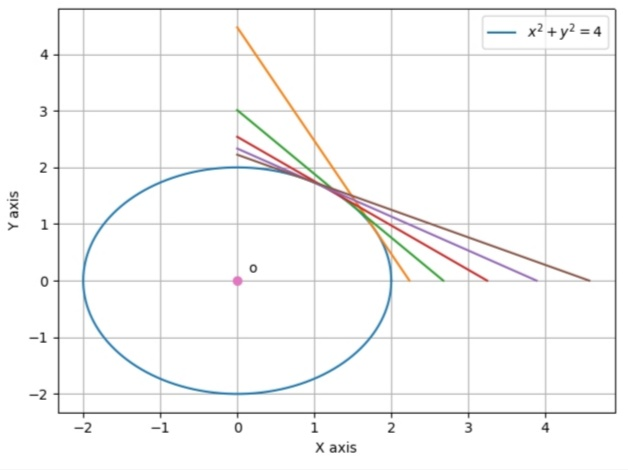
\includegraphics[scale=0.5]{figure_1-1.png}

\end{frame}




\begin{frame}
[t]{Solution}

General equation of a quadratic curve is given by 
 \vspace{0.5cm}
\hspace{1.5cm} 

$A$$x^2_1$ +$B$$x_1x_2$+$C$$x^2_2$+$D$$x_1$+$E$$x_2$ +$F$ = $0$
\vspace{0.5cm}

This can be expressed as \\
 \vspace{0.5cm}
 \hspace{1cm}
  $x^T$$V$$x$ + $2u^T$ + $F$ = $0$ 
 
 
where 
\vspace{0.5cm}

$x$ =$
\begin{bmatrix}
x\\
y
\end{bmatrix}
$
\hspace{1cm}
$V$ = $\begin{bmatrix}

A & B/2\\
B/2 & C
\end{bmatrix}$ 
\vspace{1cm}
\hspace{1cm}
$u^T$ =
$\begin{bmatrix}
D & E
\end{bmatrix}$ 
 
 
 
\end{frame}



\begin{frame}

For a circle with centre at origin
\vspace{1cm}


$V$ =
$
\begin{bmatrix}
1 & 0\\
1 & 0
\end{bmatrix}$ 
\vspace{1cm}

$u^T$ =$\begin{bmatrix}
0 & 0
\end{bmatrix}$

\vspace{1cm}

Therefrore equation of the circle $S$ is $xx^T$ - $4$ =$0$

\end{frame}


\begin{frame}

The tangent to any point $P$ on the curve is given by
\vspace{0.5cm}


$\begin{bmatrix}

P^T & 1
\end{bmatrix}
$
$\begin{bmatrix}

V & u\\
u^T & F 
\end{bmatrix}
$
$
\begin{bmatrix}
x\\
1
\end{bmatrix}
$ =0
\vspace{0.5cm}


This can be expressed as\\
\vspace{1cm}
\hspace{1cm}
$
\begin{bmatrix}
P^TV + u^T
\end{bmatrix}
$
x + $P^T$$u$ +$F$ = $0$
\vspace{1cm}

Substitute the values of $V$ and $u$

\end{frame}

\begin{frame}

Equation of tangent $MN$ is 
$P^T$x - $4$ = $0$ 
\vspace{2cm}\\
Parametric form of the circle is  
\vspace{0.5cm}\\
x = rcos$\theta$ \\
y = rsin$\theta$
\\
\hspace{4cm}  radius $r$ = 2
\end{frame}

\begin{frame}

Taking P = 
$
\begin{bmatrix}
2cos\theta\\
2sin\theta
\end{bmatrix}
$
\hspace{3cm}
$0$ $<$ $\theta$ $<$ $\pi/2$
\vspace{1cm}

$P^T$ =
$ \begin{bmatrix}
2cos\theta &
2sin\theta
\end{bmatrix}
$
\vspace{1cm}

Therefore 

$ \begin{bmatrix}
2cos\theta &
2sin\theta
\end{bmatrix}
$ $ \begin{bmatrix}
x \\y

\end{bmatrix}
$ = 4\\
\vspace{0.5cm}
Dividing by $4$ on both sides ,we get

$ \begin{bmatrix}
cos\theta/2 &
sin\theta/2
\end{bmatrix}
$ $ \begin{bmatrix}
x \\y

\end{bmatrix}
$ = 1

\end{frame}
\begin{frame}


Intercept form of a straight line :



$ \begin{bmatrix}
\frac{1}{a}&
\frac{1}{b}
\end{bmatrix}
$ $ \begin{bmatrix}
x \\y

\end{bmatrix}
$ = 1\\

\vspace{1cm}
$x$ intercept = $a$
\\
$y$ intercept = $b$
\vspace{1cm}


Comparing the the equations ,we get 

$a$ = $\frac{2}{cos\theta}$  ;
$b$ = $\frac{2}{sin\theta}$

\end{frame}

\begin{frame}

Midpoint of line segment MN = $\begin{bmatrix}

\frac{1}{cos\theta}\\\frac{1}{sin\theta}
 \end{bmatrix}$
 
 \vspace{0.4cm}
 
 
\hspace{1.5cm} $x$ = $\frac{1}{cos\theta}$
          \hspace{1.5cm}$y$ = $\frac{1}{sin\theta}$
          
        \vspace{1cm}
 
 $(cos^2\theta)$ +  $(sin^2\theta)$ = 1
 
 \vspace{1cm}
Therefore, the locus is 


\hspace{4cm}
$x^2$+$y^2$ = $x^2$$y^2$
 
 
\end{frame}
\begin{frame}
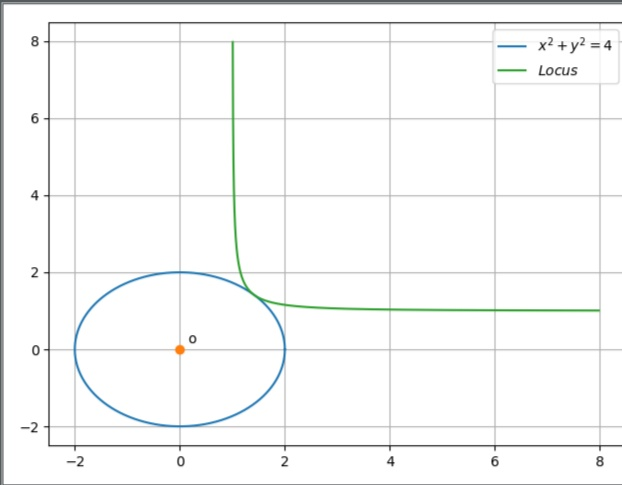
\includegraphics[scale=0.5]{figure_1-3}
\end{frame}

\end{document}